% 描述:使用LaTex做笔记的母版,建议使用Traditional或pdf编译执行。
% 编码:utf-8
% 作者:Wang Jianzhao
% 日期:2020-02-19
% ==================================================================================================================

\documentclass[UTF8, a4paper]{ctexart}

% 页面设置
	\usepackage{geometry}
	\geometry{left=3.17cm,right=3.17cm,top=2.54cm,bottom=2.54cm}
	% \setlength{\parindent}{0pt} % 设置全篇不首行缩进.
	\usepackage{indentfirst}      % 设置每章节第一段首行缩进.
	% \setlength{\parskip}{1em}   % 设置标题段间距.
	% \setlength{\lineskip}{2em}  % 设置标题段行距.

% 页眉和页脚
	\usepackage{fancyhdr}
	\pagestyle{fancy}
	\lhead{作者姓名}
	\chead{简略标题}
	\rhead{\thepage}
	\cfoot{}

% 设置全局字体(新罗马和宋体)
	\usepackage{fontspec}
	\setmainfont{Times New Roman}
	% \setCJKmainfont{SimSun}
	\CJKfamily{song}
	% \usepackage{type1cm}
	% \fontsize{30pt}{18pt}\selectfont

% 可能用得到的包
	\usepackage{xcolor}
	\usepackage{enumerate}
	\usepackage{amssymb}
	\usepackage{setspace}
	\usepackage{graphicx}
	\usepackage{subfigure}
	\usepackage{caption}
	\usepackage{subfig}
	% \usepackage[colorlinks, citecolor=blue]{hyperref}
	\usepackage{amsmath}
	\numberwithin{equation}{section} % 设置公式编号格式为不连续编号.
	\allowdisplaybreaks[4] % 跨页方程组自动分割到两页.

\newcommand{\tcr}{\textcolor{blue}}
\newcommand{\upcite}[1]{\textsuperscript{\textsuperscript{\tcr{\cite{#1}}}}}

\title{{\Huge 请在此处输入标题}}
\author{作者姓名}

\begin{document}
\maketitle

\tableofcontents % 显示目录
\newpage

% \begin{center}
% \section{Section 1}
% \end{center}
% \vspace{3ex}

% \begin{spacing}{2.0} % 设置双倍行距直到 '\end{spacing}'

\section{第一章标题}

	\begin{enumerate}
	% \begin{enumerate}[(1)]
	\item 大家好\upcite{ref1}.

	\item 大家好\cite{ref1,ref2}.

	\item 大家好.
	\end{enumerate}

\section{第二章标题}

	\textcolor{red}{大家好.}

	\subsection{第一节标题}

		图片的插入.

		\begin{figure}[h]
			\centering
			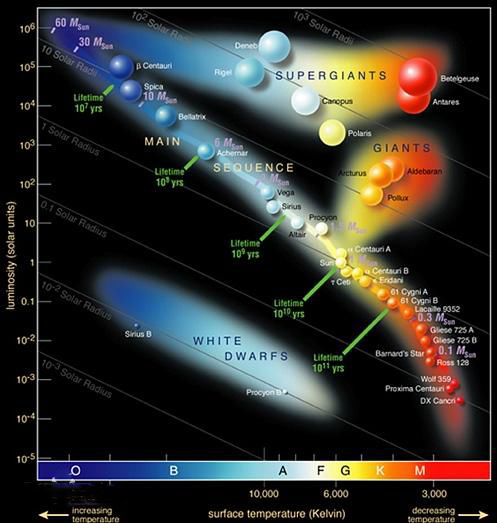
\includegraphics[width=4cm,height=5cm]{2-1.png}
			\caption{描述这是图片1.}
		\end{figure}

		\begin{figure}[ht]
			\centering
			\subfigure[图片1(a)]{
			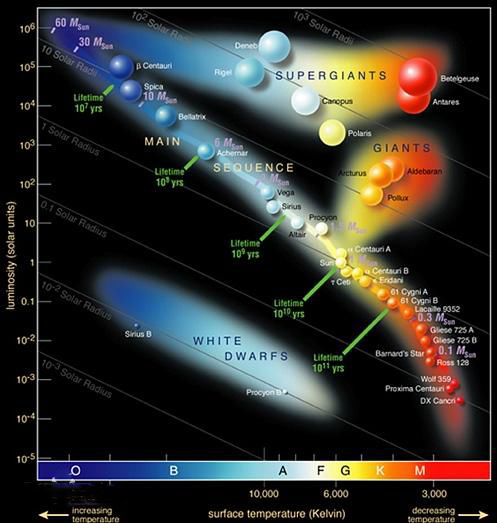
\includegraphics[width=4cm,height=5cm]{2-1.png}}
			\hspace{0in}
			\subfigure[图片1(b)]{
			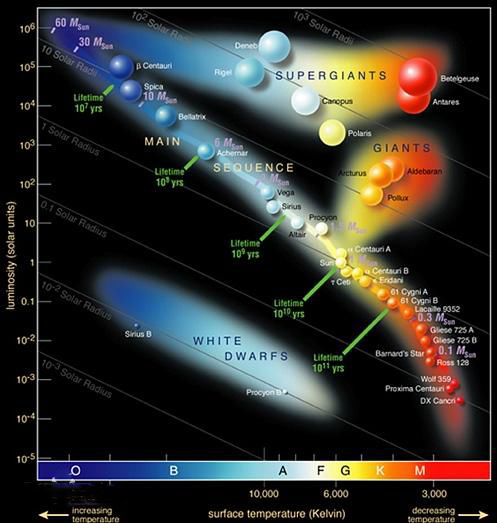
\includegraphics[width=4cm,height=5cm]{2-1.png}}
			\caption{描述这是图片 2.}
		\end{figure}

	\subsection{第二节标题}

		公式的插入.

		\begin{equation}
			\mathbf{E}=\sum_{l=0}^{\infty} \sum_{m=-l}^{l}\left(E_{l m}^{r}(r) \mathbf{Y}_{l m}+E_{l m}^{(1)}(r) \boldsymbol{\Psi}_{l m}+E_{l m}^{(2)}(r) \boldsymbol{\Phi}_{l m}\right)
		\end{equation}

		\begin{align}
			\mathbf{Y}_{l m}    & =Y_{l m}(\phi,\theta)\  \hat{\mathbf{e}}_r \\
			\notag
		    \boldsymbol{\Psi}_{l m} & =r \nabla Y_{l m}=\frac{1}{\sin \theta} \frac{\partial Y_{lm}}{\partial \phi}\hat{\mathbf{e}_{\phi}} + \frac{\partial Y_{lm}}{\partial \theta}\hat{\mathbf{e}_{\theta}} \\
		    \boldsymbol{\Phi}_{l m} & =\overrightarrow{\mathbf{r}} \times \nabla Y_{l m}=\frac{\partial Y_{lm}}{\partial \theta}\hat{\mathbf{e}_{\phi}} -\frac{1}{\sin \theta} \frac{\partial Y_{lm}}{\partial \phi}\hat{\mathbf{e}_{\theta}}
		\end{align}

	\subsection{第三节标题}

		表格的插入.

		\begin{table}[h]
			\renewcommand\arraystretch{2}
			\centering
			\caption{这是表格1.}
			\begin{tabular}{|c|c|c|c|}
				\hline \        & X & Y             & Z             \\
				\hline particle & 2 & $\frac{3}{4}$ & $\frac{1}{2}$ \\
				\hline ion      & 1 & $\frac{1}{4}$ & 0             \\
				\hline electron & 1 & $\frac{2}{4}$ & $\frac{1}{2}$ \\
				\hline
			\end{tabular}
		\end{table}

% \section{第三章}

% 参考文献.

	\begin{thebibliography}{99} 
	\addcontentsline{toc}{section}{参考文献} 
		\bibitem{ref1}Zheng L, Wang S, Tian L, et al., ApJ, 2015: 1741-1750.  
		\bibitem{ref2}Arandjelov R, Zisserman A, IEEE, 2012: 2911-2918.  
	\end{thebibliography}

% \end{spacing}

\end{document}
